\documentclass[11pt]{article} % For LaTeX2e
\usepackage{rldmsubmit,palatino}
\usepackage{graphicx}
\usepackage{natbib}

\title{Escaping Groundhog Day}


\author{}

% The \author macro works with any number of authors. There are two commands
% used to separate the names and addresses of multiple authors: \And and \AND.
%
% Using \And between authors leaves it to \LaTeX{} to determine where to break
% the lines. Using \AND forces a linebreak at that point. So, if \LaTeX{}
% puts 3 of 4 authors names on the first line, and the last on the second
% line, try using \AND instead of \And before the third author name.

\newcommand{\fix}{\marginpar{FIX}}
\newcommand{\new}{\marginpar{NEW}}

\begin{document}

\maketitle

\begin{abstract}
Existing approaches to reinforcement learning rely on a fixed
state-action space and reward function that the agent is trying to
maximize.  During training, the agent is repeatedly reset to a
predefined initial state or set of initial states.  For example, in
the classic RL Mountain Car domain, the agent starts at some point in
the valley, continues until it reaches the top of the valley and then
resets to somewhere else in the same valley. Learning in this regime
is akin to the learning problem faced by Bill Murray in the 1993 movie
{\em Groundhog Day} in which he repeatedly relives the same day, until
he discovers the optimal policy and escapes to the next day.  In a
more realistic formulation for an RL agent, every day is a new day
that may have similarities to the previous day, but the agent never
encounters the same state twice.  This formulation is a natural fit
for robotics problems in which a robot is placed in a room in which it
has never previously been, but has seen similar rooms with similar
objects in the past.  We formalize this problem as learning to act in
a {\em domain}. A domain is defined by the tuple $(X, A, P)$, where
$X$ is a state representation, $A$ is an action set, and $P$ is a
probability distribution of MDPs with different state spaces, reward
functions, and transition dynamics, but the same state representation
$X$ and action set $A$. The agent samples an MDP from some unknown
distribution of related MDPs and must learn to behave well under the
distribution of MDPs. The agent observes samples from the MDP
distribution and at test time is evaluated on a new set of MDP samples
drawn from the same distribution, focusing the evaluation on the
agent's ability to generalize.



%% In this setting there are two key problems: (1) learning
%% to plan and (2) learning to learn. In learning to plan, the agent
%% always knows the transition dynamics for each MDP; however, the agent
%% can exploit its knowledge from solving previous MDPs from the
%% distribution to more efficiently find good solutions in new MDPs. In
%% learning to learn, the agent does not know the transition dynamics for
%% each MDP, but can use knowledge from learning in previous MDPs to
%% learn a portable model or bias its exploration through the state
%% space. 

%% In principle, $P$ could have such a large variation
%% that nothing learned in one MDP drawn from it is useful for another;
%% however, we are interested in domains in which there strong
%% commonalities. For example, in the real world, no two rooms may be the
%% same, but physical and social constraints entail similarity in the
%% mechanics of objects such as light switches and door knobs; we would
%% like are agent to learn in this types of scenarios.

%In the 1993 movie {\em Groundhog Day}, Bill Murray plays a character, Phil, who suddenly finds himself forced to repeatedly relive the same day. Regardless of whether he stays up all night, or even dies, by what would be the next day's start, he is back in bed at the beginning of the day he just lived. By repeating the same day, Phil is able to learn how to accomplish amazing feats in that day that no other human would otherwise be able to accomplish without similarly being able to re-experience the same events. Groundhog Day is interesting precisely because it places the protagonist in such a recognizably unrealistic situation, yet AI research in reinforcement learning (RL) is typically more similar to Groundhog Day than it is to learning how to behave in real life. In RL, agents are dropped into a state of an environment, allowed to act in it for some length of time or until a terminal state is reached, and then are reset back to the beginning of the same environment again.

%Although studying RL in the context of a single environment has been an excellent starting point for research with a number of applications, it has a number of limitations that prevent algorithms from scaling to many real world problems. For example, suppose we wish to develop an assistant robot that can be deployed to any number of homes. Tuning a learning algorithm to behave in a well defined home environment is likely to lead to both forms of overfitting and underfitting. Overfitting can occur because we do not expect every home to be the same nor reset itself each day. Underfitting can occur if the agent does not generalize experience in one environment to new environments. In response to these limitations, we advocate for a problem formulation in which the agent must learn how to behave well in a distribution of environments from a sequence of environments drawn from the same distribution. We review existing work that can be adapted to this paradigm and highlight challenges to be addressed.

\end{abstract}

\keywords{
Meta-learning, transfer learning, learning to plan,
}



\startmain % to start the main 1-4 pages of the submission.

\section{Introduction}
The dominant approaches to reinforcement learning rely on a fixed
state-action space and reward function that the agent is trying to
maximize.  During training, the agent is repeatedly reset to a
predefined initial state or set of initial states.  For example, in
the classic RL Mountain Car domain, the agent starts at some point in
the valley, continues until it reaches the top of the valley and then
resets to somewhere else in the same valley. Learning in this regime
is akin to the learning problem faced by Bill Murray in the 1993 movie
{\em Groundhog Day} in which he repeatedly relives the same day, until
he discovers the optimal policy and escapes to the next day.  In a
more realistic formulation for an RL agent, every day is a new day
that may have similarities to the previous day, but the agent never
encounters the same state twice.  This formulation is a natural fit
for robotics problems in which a robot is placed in a room in which it
has never previously been, but has seen similar rooms with similar
objects in the past. We formalize this problem as optimizing a learning or planning
algorithm for a set of environments drawn from a distribution.

In both cases, we assume environments are defined by a Markov decision process (MDP). An MDP is defined by the tuple $(S, A, T, R, s_0)$, where $S$ is the state space; $A$ is the action set; $T(s' | s, a)$ is the transition dynamics, which specifies the probability of transitioning to state $s'$ after taking action $a$ in state $s$; $R(s, a, s')$ is the reward function, which specifies the reward received by the agent for taking action $a$ in state $s$ and then transitioning to state $s'$; and $s_0$ is an initial state.

The goal of planning or learning in an MDP is to find a (near-)optimal policy $\pi$ that maps states to actions. A policy is typically considered optimal if following it from the initial state maximizes the expected discounted future reward.
%$E \left[ \sum_{t=0}^{\infty} \gamma^t r_t \mid s_0, \pi \right]$, where $\gamma \in [0, 1]$ is a discount factor specifying how much the agent prefers immediate rewards over more distant rewards and $r_t$ is the reward received at time $t$. 
In a planning problem, the agent has complete access to the MDP and can search for a policy before acting in the world. In reinforcement learning (RL), the agent does not have access to the transition dynamics or reward function and must learn how to act through interaction with the environment.

In our learning setting, an agent is given a set of sample training MDPs on which to optimize its performance. In the case of planning, learning from the training set is used to decrease planning computation time in future environments. In RL, learning from the training set is used to decrease learning time in new environments.

We present results for the learning to plan and learning to learn setting. In the learning to plan setting we present learnable \emph{goal-based action priors} that accelerate planning on related MDPs. In the learning to learn setting, we present \emph{sample-optimized Rademacher complexity},
which is a formal mechanism for assessing the risk in choosing a learning algorithm tuned on a training set drawn from the distribution for use on the entire distribution.

\section{Learning to Plan}

Robots operating in unstructured, stochastic environments such as a
factory floor or a kitchen face a difficult planning problem due to
the large state space and the very large set of possible
tasks~\citep{bollini12,knepper13}.  A powerful and flexible robot such
as a mobile manipulator in the home has a very large set of possible
actions, any of which may be relevant depending on the current goal
(for example, robots assembling furinture~\citep{knepper13} or baking
cookies~\citep{bollini12}.)  When a robot is manipulating objects in
an environment, an object can be placed anywhere in a large set of
locations.  The size of the state space increases exponentially with
the number of objects, which bounds the placement problems that the
robot is able to expediently solve.  Depending on the reward function
(which is unknown before runtime), any of these states and actions may
be relevant to the solution, but for any specific reward function,
most of them are irrelevant.  For instance, when making brownies, the
oven and flour are important, while the soy sauce and saut\'{e} pan
are not.  For a different task, such as stir-frying broccoli, the
robot must use a different set of objects and
actions. 
\begin{figure}
\centering
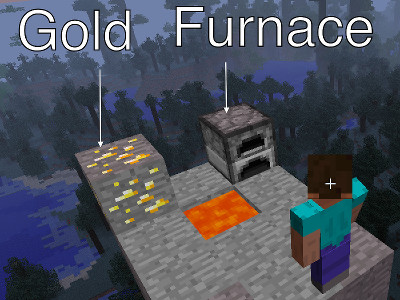
\includegraphics[width=0.25\linewidth]{figures/smelt_small.jpg}
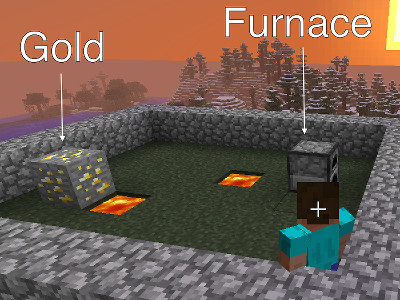
\includegraphics[width=0.25\linewidth]{figures/smelt_large.jpg}
\caption{Two different problems from the same domain, where the
  agent's goal is to smelt the gold in the furnace while avoiding the
  lava.  Our agent is unable to solve the problem on the right before
  learning because the state/action space is too large (since it can
  place the gold block anywhere).  After learning, it can quickly
  solve the larger problem.\label{fig:example}}
\end{figure}

To confront this state-action space explosion, prior work has explored
adding knowledge to the planner, such as options~\cite{sutton99} and
macro-actions~\cite{Botea:2005kx,Newton:2005vn}.  However, while these
methods can allow the agent to search more deeply in the state space,
they add non-primitive actions to the planner which {\em increase} the
branching factor of the state-action space.  The resulting augmented
space is even larger, which can have the paradoxical effect of
increasing the search time for a good policy~\cite{Jong:2008zr}.
Deterministic forward-search algorithms like hierarchical task
networks (HTNs)~\citep{Nau:1999:SSH:1624312.1624357}, and temporal
logical planning
(TLPlan)~\citep{Bacchus95usingtemporal,Bacchus99usingtemporal}, add
knowledge to the planner that greatly increases planning speed, but do
not generalize to stochastic domains. Additionally, the knowledge
provided to the planner by these methods is quite extensive, reducing
the agent's autonomy and must be manually supplied by the designer.

To address these issues, we augment an Object Oriented Markov Decision
Process (OO-MDP) with a specific type of action prior conditioned on
the current state and an abstract goal description.  Because we
condition on both the state and goal description, we refer to this
goal-based action prior as a knowlege base of {\em affordances}.  We
rigorously formalize the notion of affordances as a prior on actions
conditioned on features of the current state as well as the robot's
goal.  Affordances enable the robot to prune irrelevant actions on a
state-by-state basis based on the agent's current goal and focus on
the most promising parts of the state space.  Affordances can be
specified by hand or alternatively learned through experience in
related problems, making them a concise, transferable, and learnable
means of representing useful planning knowledge. Our experiments
demonstrate that affordances provide dramatic improvements for a
variety of planning tasks compared to baselines in simulation, and are
applicable across different state spaces.  Moreover, while manually
provided affordances outperform baselines, affordances learned through
experience yield even greater improvements.We conduct experiments in
the game Minecraft, which has a very large state-action space, and on
a real-world robotic cooking assistant.  Figure~\ref{fig:example}
shows an example of two problems from the same domain in the game
Minecraft; the agent learns on randomly generated problems and tests
on new problems from the same domain that it has never previously
encountered.


To learn affordances, we provide a set of training worlds from the
domain ($W$), for which the optimal policy, $\pi$, may be tractably
computed using existing planning methods. Then, we compute the maximum
likelihood estimate of the parameter vector $\theta_i$ for each action
using the policy.  During the learning phase, the agent learns which
actions are useful under different conditions. At test time, the agent
will see different, randomly generated worlds from the same domain,
and use the learned affordances to increase its speed at inferring a
plan.  For simplicity, our learning process uses a strict separation
between training and test; after learning is complete our model
parameters remain fixed.

We evaluate our approach using the game Minecraft.  Minecraft is a 3-D
blocks game in which the user can place, craft, and destroy blocks of
different types.  Minecraft's physics and action space allow users to
create complex systems, including logic gates and functional
scientific graphing
calculators\footnote{https://www.youtube.com/watch?v=wgJfVRhotlQ}.
Minecraft serves as a model for robotic tasks such as cooking
assistance, assembling items in a factory, object retrieval, and
complex terrain traversal.  Figure~\ref{fig:example} shows two scenes
from Minecraft.  Our experiments consisted of five common tasks in
Minecraft, including constructing bridges over trenches, smelting
gold, tunneling through walls, basic path planning, and digging to
find an object.  We tested on randomized worlds of varying size and
difficulty. The generated test worlds varied in size from tens of
thousands of states to hundreds of thousands of states.  The agent
learned affordances from a training set consisting of 25 simple state
spaces of each map type (100 total maps), each approximately a
1,000-10,000 state world. We conducted all tests with a single
knowledge base. Learning this knowledge base took approximately one
hour run in parallel on a computing grid.


We use Real-Time Dynamic Programming (RTDP)~\cite{barto95} as our
baseline planner, a sampling-based algorithm that does not require the
planner to visit all states. We compare RTDP with learned
affordance-aware RTDP (LA-RTDP), and expert-defined affordance-aware
RTDP (EA-RTDP). We terminated each planner when the maximum change in
the value function was less than 0.01 for 100 consecutive policy
rollouts, or the planner failed to converge after 1000 rollouts.  The
reward function was $-1$ for all transitions, except transitions to
states in which the agent was in lava, where we set the reward to
$-10$. The goal was set to be terminal and the discount factor was
$\gamma = 0.99$.  To introduce non-determinism into our problem,
movement actions (move, rotate, jump) in all experiments had a small
probability (0.05) of incorrectly applying a different movement
action.  This noise factor approximates noise faced by a physical
robot that attempts to execute actions in a real-world domain and
can affect the optimal policy due to the existence of lava pits
that the agent can fall into. 


% -- Figure: Average results --
\begin{figure}[t]
%\begin{figure}
\centering
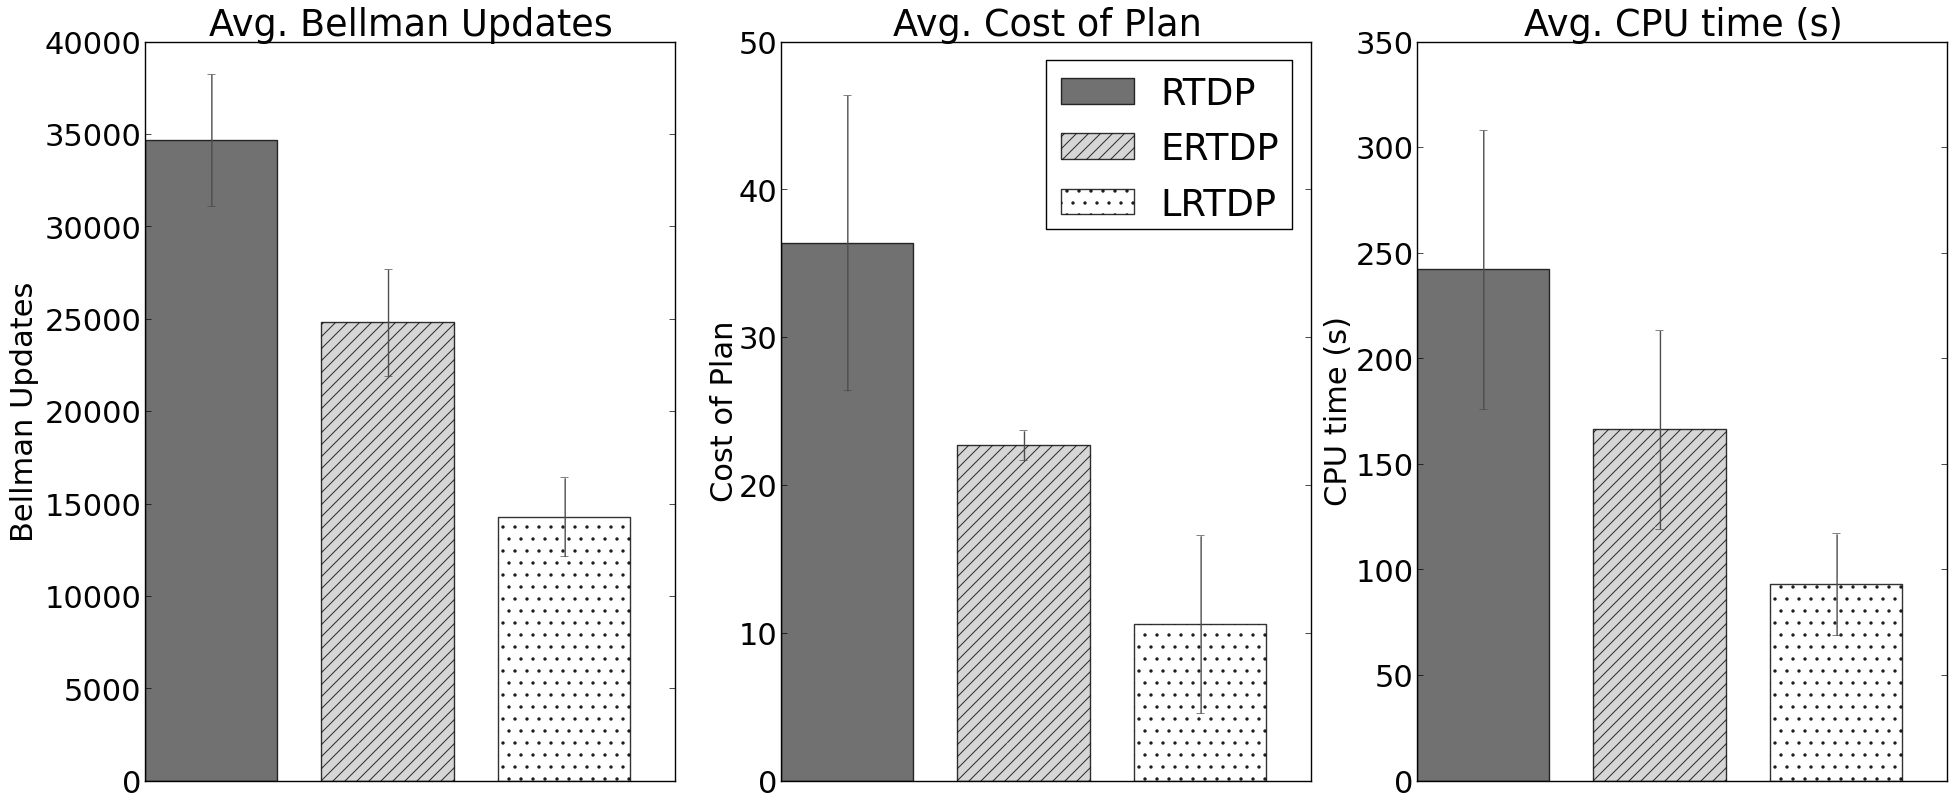
\includegraphics[width=0.3\linewidth]{figures/average_results_cropped.png}%
%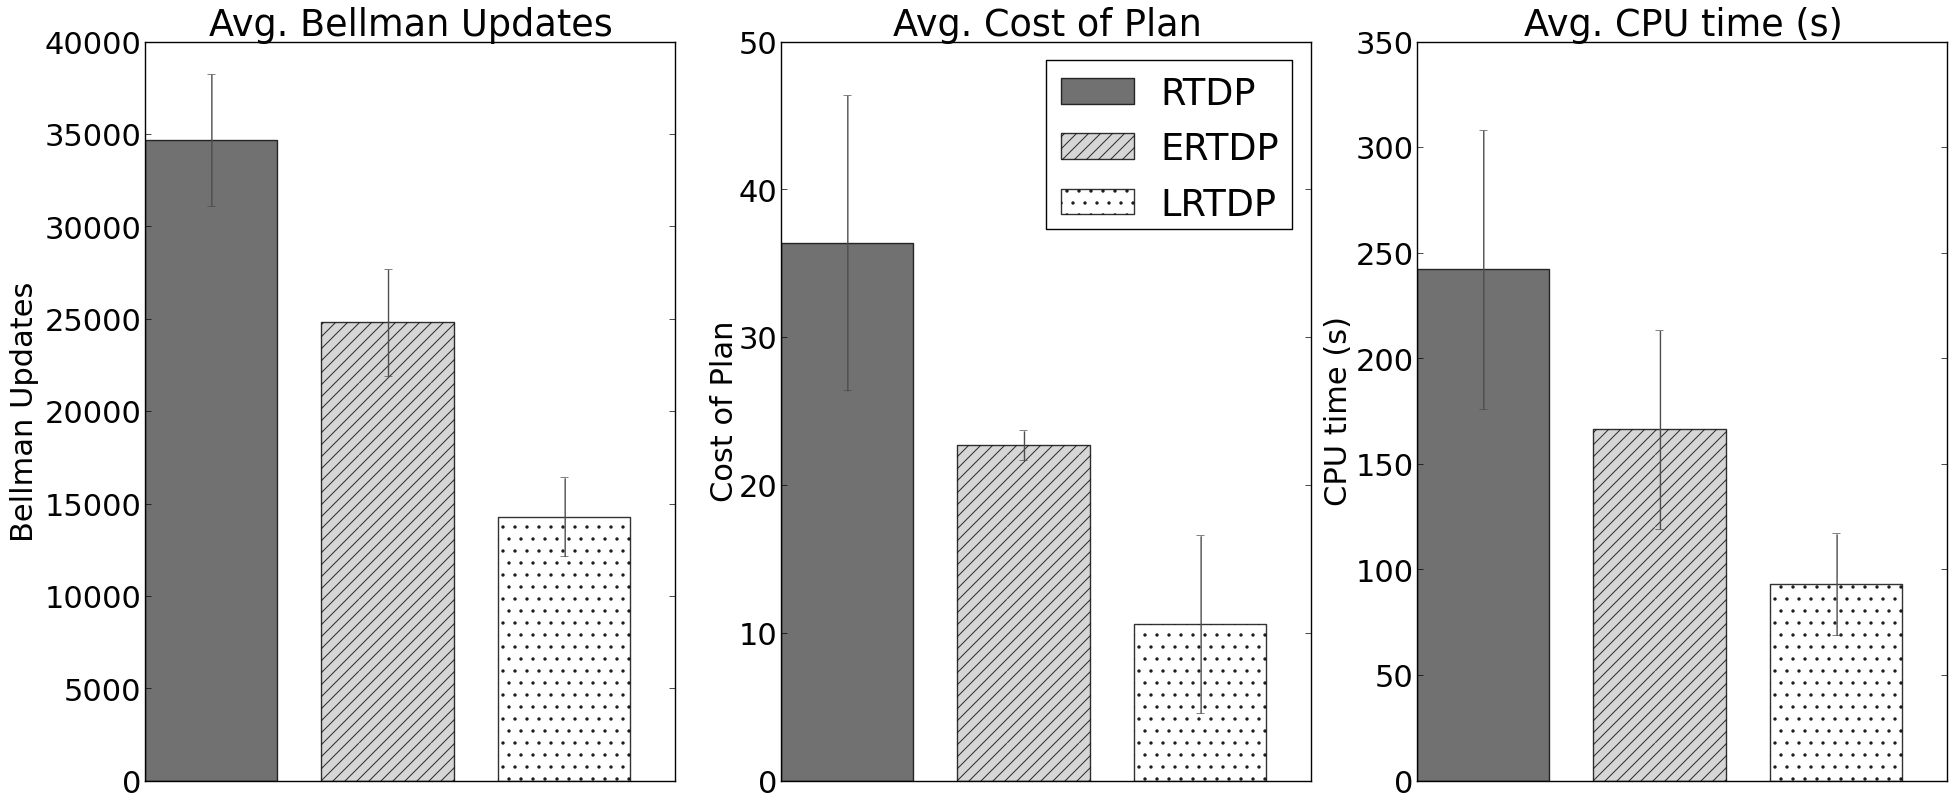
\includegraphics[scale=0.18]{figures/average_results_cropped.png}%
\caption{Average results from all maps.}
\label{fig:average_results}
\end{figure}
%\end{figure}



\section{Learning to Learn}
For the case of optimizing a learning algorithm for a distribution of MDPs, we seek to answer the question: How do you know if your reinforcement-learning (RL) algorithm is the right one for your problem? How can you tell if you are at risk for overfitting? Or underfitting?

%Overfitting is the phenomenon in which a learning method optimizes itself to noise in its training examples and is therefore likely to miss the function that best generalizes to new data. Recognized as a central problem in supervised machine learning~\cite{Mitchell:1997:ML:541177}, the problem also appears in other optimization settings such as choosing the best optimizer for a class of problems~\cite{DBLP:journals/jmlr/YoonFG08,sorg2010internal}
%aaai-fall-peter, Polya1956
%or choosing the right RL approach for a family of tasks~\cite{dabney13,nouri09,Whiteson11}. It is this latter problem we seek to formalize here. 

A core concept used in mitigating the effects of overfitting is to apply more powerful hypothesis classes only when copious data is available to fit their free parameters, restricting learners to weaker hypothesis classes when data is more sparse. In some well-studied cases, bounds relating the hypothesis class to the amount of data required to fit it accurately are known~\cite{blumer1989learnability}. 
%In this paper, we provide a formal procedure for making estimates even in the context of considerably more complex hypothesis classes for which analytical results are unknown and use it in the context of RL.

As an example, consider the 5-state chain~\cite{strens2000bayesian}: a well known Markov decision process (MDP).
%The MDP is the 5-state chain~\cite{strens2000bayesian}. 
This problem consists of a set of 5 states arranged in a linear order. Action $a_1$ causes a transition to the next state in the ordering. Action $a_2$ resets the state to the first in the chain. Action $a_1$ from the last state in the chain results in remaining in the state with a high reward ($+10$) and zero reward otherwise. Action $a_2$ always has a reward of $+2$. %Rewards are discounted, $\gamma=0.95$. 
With probability $0.2$ (the slip probability), however, the selected action has the effect of the non-selected action. Though tiny, this MDP is challenging for some learning algorithms because action $a_2$ acts as a temptation that keeps the agent from discovering the optimal policy (always take action $a_1$). We measure the performance of a learning algorithm in the environment by its probability of finding an optimal policy after 1000 steps of experience. 

Consider two different variations of the Q-learning algorithm~\cite{sutton1998reinforcement} that we might want to apply to this problem. In both, the learning rate ($\alpha$) is set to a value between $0.0$ and $0.5$ and the exploration rate ($\epsilon$) is set to a value between $0.0$ and $0.4$.
% , \edit{uniformly at random}.
In the \emph{constant initialization} algorithm, all Q values are initially set to %some value between $0$ and $200$. 
$45$ (something in the vicinity of the likely final value function).
In the \emph{variable initialization} algorithm, each state--action pair is initialized independently to some value between $0$ and $200$. Note that the variable initialization algorithm subsumes the constant initialization algorithm since it can be configured to initially set all Q values to 
%the same number.  explain actual algorithms we used
$45$.

If we tune parameters to the 5-state chain MDP, the variable initialization algorithm will perform better. However, that does not mean the tuned variable initialization algorithm will perform better on a distribution of varying 5-state chain problems, depending on the properties of the distribution. For example, consider two different MDP distributions. In distribution~1, all MDPs are 5-state chains with states ordered consistently but slip probability varying between $0.19$ and $0.21$. In distribution~2, all MDPs are 5-state chains, with the order of states in the chain varying from MDP to MDP and slip probability varying between $0.00$ and $0.50$. By exhaustive testing shown in Figure~\ref{fig:underfit}, we find that for distribution~1, tuning variable initialization on a single MDP results in a training performance comparable to performance across the entire distribution. However, for distribution~2, the training performance of variable initialization on a single MDP is deceptive and constant initialization performs better on the full distribution. That is, variable initialization overfits. %to the single training example. 
As more training samples for distribution~2 are provided, overfitting is mitgated and variable initialization
is the better choice.
%variable initialization's training performance becomes more reflective of its performance on the full distribution and is the better choice.
\begin{figure*}
\centering
\begin{tabular}{cc}
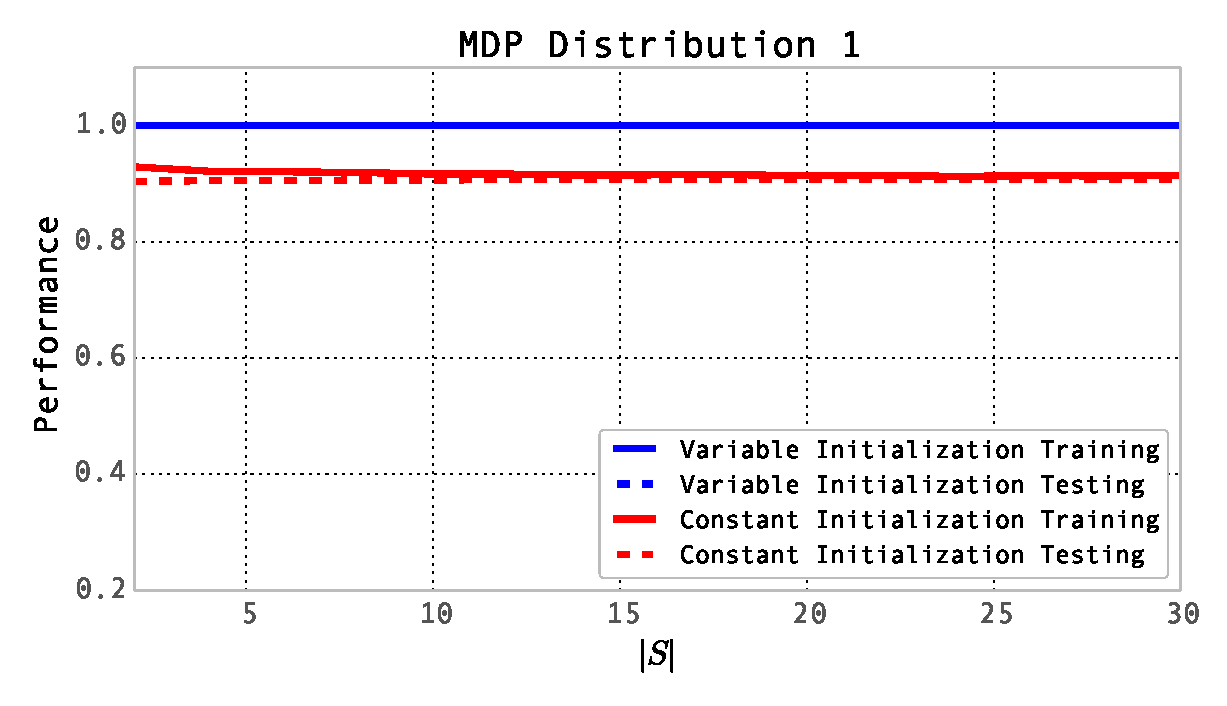
\includegraphics[width=.4\columnwidth]{images/mdp_distribution1} &
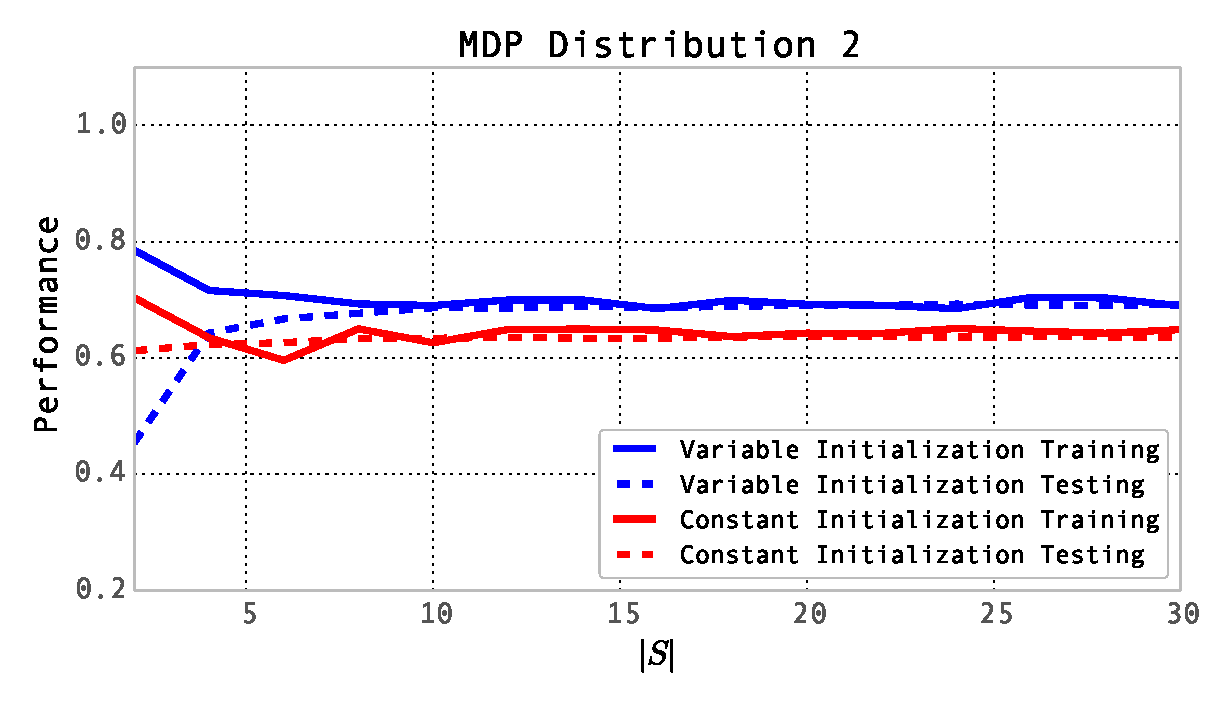
\includegraphics[width=.4\columnwidth]{images/mdp_distribution2}
\end{tabular}
\caption{Training and testing performance for two distributions in the 5-state chain environment.} %Performance is measured as the probability of converging to the optimal policy.}
\label{fig:underfit}
\end{figure*}

Since performance on the training set of MDP samples can be deceptive, we would like a way to bound the {\em generalization error}. The generalization error is the difference in the performance of a selected algorithm on a training set and its performance on the full distribution. More formally, let $\mathcal{A}$ be the space of parameterized algorithms and let $\mathcal{F}$ be the space of evaluation functions of each algorithm $a \in \mathcal{A}$ such that for all $f_a \in \mathcal{F}$, $f_a : \mathcal{D} \rightarrow [0,1]$, where $\mathcal{D}$ is the space of MDPs our MDP distribution spans. Let $S$ be a sample $z_1,\dots, z_m$, chosen from a distribution $D$ on $\mathcal{D}$. Then the generalization error of algorithm $a$ is $| \hat{E}_S[f_a] - E[f_a] |$, where $\hat{E}_S[f_a]= \frac{1}{m}\sum_{i=1}^m f_a(z_i)$ is the expected performance of $a$ on the training data, and $E[f_a]= \int_\mathcal{D} f_a(z) D(z) dz$ is the expected performance of $a$ on the full distribution.

A major uniform convergence result for Rademacher complexity~\cite{mohri2012foundations} states that with probability $1-\delta$ over choices of $S$,
for every function $f\in \mathcal{F}$, we have 
$E[f(z)] \le \hat{E}_S[f] + 2 R_S(\mathcal{F}) + 3\sqrt{\frac{\ln(2/\delta)}{2m}}$,
where
$R_S (\mathcal{F}) = E_{\bar{\sigma}} [\sup_{f \in \mathcal{F}} (\frac{1}{m} \sum_{i=1}^m f(z_i) \sigma_i )],$
is the emprical Rademacher complexity, and $\bar{\sigma}=(\sigma_1,\dots, \sigma_m)$ is a vector of $m$ independent random variables, with $Pr(\sigma_i =1)=Pr(\sigma_i = -1)=1/2$. The role of the $\sigma$ variables is to create a kind of output noise in the dataset.

Unfortunatley, the $\sup$ operator requires exhuastive search over all possible learning algorithms, which is generally intractable. Our main result is a new generalization bound for when the $\sup$ operator is replaced with a tractable weak form of optimization. Specifically, the weak optimization we use is to generates an ensemble of $l$ learning algorithms. This ensemble is produced by selecting $l$ subsets of $A$, each of size $k$ and for each subset choosing the maximum performing algorithm. At test time, the agent would then randomly select one of the winning $l$ algorithms for use.

Under this weak form optimization, we now have the following generalization error bound.
With probability $1-\delta$
$$E_{{F_k}}[ E_z[f^k_S] - \hat{E}_S[f^k_S] ] \leq \frac{2}{\ell} \sum_{j=1}^\ell R_S(F^j_k)+ 5\sqrt{\frac{\ln (3/\delta)}{2m}},$$
where $F_k^j$ is the set of $k$ evaluation functions for the $k$ algorithms of the $j$th subset used to form our ensemble. Due to space constraints, we have omitted the proof of this theorem.

Using this weak form of optmization, we can now compute generalization error bounds for our training data. Figure~\ref{fig:d1_750} shows how our estimated error bound in the 5-state chain problems using our weak optimizer tracks the true performance on the full distribution. It correctly predicts that on distribution~1 variable initialization should be prefered even with only one training sample, but on distribution~2, constant initialization should be preferred at first. The conservative nature of the bounds means that there is a need for a large training set before they can be convinced that variable initialization is not overfitting. Fortunately, the two sets of algorithm have similar performance after a handful of training samples.
\begin{figure*}
\centering
\begin{tabular}{cc}
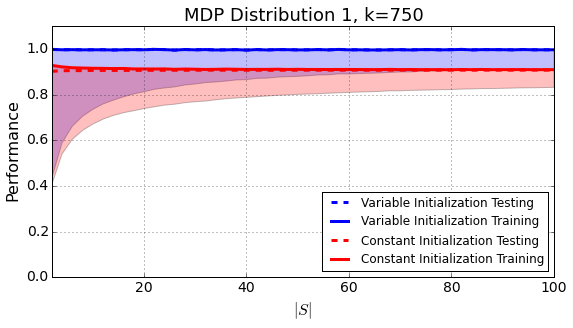
\includegraphics[width=.4\columnwidth]{images/mdp_distribution1_sampled_rademacher_k_750} &
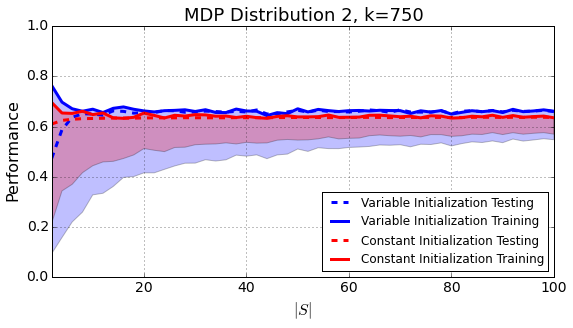
\includegraphics[width=.4\columnwidth]{images/mdp_distribution2_sampled_rademacher_k_750}
\end{tabular}
\caption{Generalization error for 5-state chain Distributions~1 and~2 using an ensemble of $l=20$ learning algorithms, each chosen from a subset of $k=750$ learning algorithms.}
\label{fig:d1_750}
\end{figure*}


%\section{Conclusion}

\bibliographystyle{plain}
{\small
\bibliography{groundhog,main}
}


\end{document}
